\documentclass{scrreprt}

\usepackage{aligned-overset}
\usepackage{amsmath}
\usepackage{amsthm}
\usepackage{amssymb}
\usepackage{bm}
\usepackage[shortlabels]{enumitem}
\usepackage{hyperref}
\usepackage[utf8]{inputenc}
\usepackage{multicol}
\usepackage{mathtools}
\usepackage{pdflscape}
\usepackage{physics}
\usepackage{polynom}
\usepackage{tabularx}
\usepackage[table]{xcolor}
\usepackage{titling}
\usepackage{fancyhdr}
\usepackage{xfrac}
\usepackage{pgfplots}

\pgfplotsset{compat = newest}
\usetikzlibrary{arrows, arrows.meta}
\usetikzlibrary{calc}

\author{Karsten Lehmann \\ 4935758}
\date{WiSe 2024/25}
\title{Nachbereitungsaufgaben 6\\INF-B-110, Diskrete Strukturen}

\setlength{\headheight}{26pt}
\pagestyle{fancy}
\fancyhf{}
\lhead{\thetitle}
\rhead{\theauthor}
\lfoot{\thedate}
\rfoot{Seite \thepage}

\newcommand{\ggT}[0]{\text{ggT}}
\DeclarePairedDelimiter{\floor}{\lfloor}{\rfloor}

\begin{document}
\paragraph{N6}
\begin{enumerate}[(a)]
\item Es sind die komplexen Zahlen
  $z_k \coloneqq e^{\frac{\pi}{3}ki}, k = 0, \ldots, 5$ gegeben.
  Sie dürfen als bekannt voraussetzen, dass die Menge
  $G \coloneqq \qty\big{z_0, \ldots, z_5}$  mit der üblichen Multiplikation
  komplexer Zahlen eine Gruppe bildet.
  \begin{enumerate}[(1)]
  \item Berechnen Sie $z_5 \cdot z_4 \in G$. (Zeigen Sie die Rechnung im Detail)

    \subparagraph{Lsg.} Es sind $z_5 = e^{\frac{\pi}{3}5i}$ und
    $z_4 = e^{\frac{\pi}{3}4i}$.

    Nun ist
    \begin{flalign*}
      z_5 \cdot z_4 &= e^{\frac{\pi}{3}5i} \cdot e^{\frac{\pi}{3}4i} \\
                    &= e^{\frac{\pi}{3}5i + \frac{\pi}{3}4i} \\
                    &= e^{\frac{9\pi}{3}i} \\
                    &= e^{\frac{3\pi}{3}i + \frac{6\pi}{3}i} \\
                    &= e^{\frac{3\pi}{3}i} \cdot \underset{=1}{\underbrace{e^{2\pi i}}} \\
                    &= e^{\frac{\pi}{3}3i} = z_3
    \end{flalign*}

  \item Stellen Sie die Verknüpfungstafel von $\qty\big(G; \cdot)$ auf.
    (Hier müssen keine Begründungen oder Rechnungen angegeben werden)

    \subparagraph{Lsg.}\label{n6_a_2}\phantom{\null}

    \begin{tabular}{|c|cccccc|}
      \hline
      $\cdot$ & $z_0$ & $z_1$ & $z_2$ & $z_3$ & $z_4$ & $z_5$ \\
      \hline
      $z_0$ & $z_0$ & $z_1$ & $z_2$ & $z_3$ & $z_4$ & $z_5$ \\
      $z_1$ & $z_1$ & $z_2$ & $z_3$ & $z_4$ & $z_5$ & $z_0$ \\
      $z_2$ & $z_2$ & $z_3$ & $z_4$ & $z_5$ & $z_0$ & $z_1$ \\
      $z_3$ & $z_3$ & $z_4$ & $z_5$ & $z_0$ & $z_1$ & $z_2$ \\
      $z_4$ & $z_4$ & $z_5$ & $z_0$ & $z_1$ & $z_2$ & $z_3$ \\
      $z_5$ & $z_5$ & $z_0$ & $z_1$ & $z_2$ & $z_3$ & $z_4$ \\
      \hline
    \end{tabular}

  \item Geben Sie alle Elemente von $G$ an, die zu sich selbst invers sind.

    \paragraph{Lsg.} Es ist $z_0 \in G$ das Neutrale Element, da für $g \in G$
    gilt $g \cdot z_0 = z_0 \cdot g = g$.

    Somit ist $h \in G$ zu sich selbst invers, wenn $h \cdot h = z_0$.

    Aus \hyperref[n6_a_2]{Teilaufgabe (2)} können nun die Elemente $z_0$ und
    $z_3$ als zu sich selbst invers abgelesen werden.

  \end{enumerate}

\newpage
\item Betrachtet wird die Menge
  $7\mathbb{Z} \coloneqq \qty\big{7k \:\big|\: k \in \mathbb{Z}}$ aller
  Vielfachen der Zahl $7$.
  Zeigen Sie, dass $\qty\big(7\mathbb{Z};+)$ (mit der üblichen Addition in
  $\mathbb{Z}$) eine Gruppe bildet.

  \subparagraph{Lsg.} Da $\mathbb{Z}$ bezüglich der Multiplikation abgeschlossen
  ist, ist $7 \cdot k \in \mathbb{Z}$ für jedes $k \in \mathbb{Z}$.
  Somit ist $7\mathbb{Z} \subseteq \mathbb{Z}$.

  Da $\qty\big(\mathbb{Z}; +)$ eine Gruppe ist, reicht es zu zeigen, dass
  $\qty\big(7\mathbb{Z};+)$ eine Untergruppe ist.

  \begin{enumerate}[(1)]
  \item es ist $0$ das neutrale Element von $\qty\big(\mathbb{Z}; +)$ und
    da $7 \cdot 0 = 0$, ist auch $0 \in \qty\big(7\mathbb{Z};+)$

  \item Sei $z \in 7\mathbb{Z}$ beliebig.
    Dann existiert $k \in \mathbb{Z}$ mit $7 \cdot k = z$.
    Da $\qty\big(\mathbb{Z}; +)$ eine Gruppe ist, existiert auch
    $-k \in \mathbb{Z}$ mit $\qty\big(-k) + k = k + \qty\big(-k) = 0$.

    Sei nun $-z = 7 \cdot \qty\big(-k)$.
    Dann ist $-z \in 7\mathbb{Z}$ und
    \[
      z + \qty\big(-z)
      = 7 \cdot k + 7 \cdot \qty\big(-k)
      = 7 \cdot \qty\big(k + \qty\big(-k))
      = 7 \cdot 0
      = 0
    \]
    Da $z$ beliebig, ist $\qty\big(7\mathbb{Z};+)$ unter $^{-1}$ abgeschlossen.

  \item Seien $z_1, z_2 \in 7\mathbb{Z}$ beliebig.
    Dann existieren $j, k \in \mathbb{Z}$ mit $7 \cdot j = z_1$ und
    $7 \cdot k = z_2$.
    Nun ist
    \[
      z_1 + z_2 = 7 \cdot j + 7 \cdot k
      = 7 \cdot \qty\big(j + k)
    \]
    und da $\qty\big(\mathbb{Z}; +)$ als Gruppe bezüglich der Addition
    abgeschlossen ist, ist auch $\qty\big(j + k) \in \mathbb{Z}$ sowie
    $7 \cdot \qty\big(j + k) \in 7\mathbb{Z}$.

    Da $z_1, z_2$ beliebig, ist $\qty\big(7\mathbb{Z};+)$ bezüglich der Addition
    abgeschlossen.
  \end{enumerate}

  $\Rightarrow \qty\big(7\mathbb{Z};+)$ ist eine Untergruppe von
  $\qty\big(\mathbb{Z}; +)$ und jede Untergruppe ist selbst wieder eine Gruppe.

\item Berechnen Sie das multiplikative Inverse des Elementes $z = 13$ in
  $\mathbb{Z}_{36}$.
  Verwenden Sie dazu den erweiterten euklidischen Algorithmus.

  \subparagraph{Lsg.} Es ist $\ggT\qty\big(13, 36) = 1$ und nun werden
  mit dem erweiterten Euklidischen Algorithmus $a, b \in \mathbb{Z}$
  gesucht mit $1 = a \cdot 13 + b \cdot 36$.

  Nun ist
  \begin{flalign*}
    36 &= 2 \cdot \underline{13} + 10 \\
    13 &= 1 \cdot \underline{10} + 3 \\
    10 &= 3 \cdot \underline{3} + 1 \\
    3 &= 3 \cdot 1 + 0
  \end{flalign*}
  und weiter
  \begin{flalign*}
    1 &= 1 \cdot 10 - 3 \cdot 3 \\
      &= 1 \cdot 10 - 3 \cdot \qty\big(13 - 10) \\
      &= 4 \cdot 10 - 3 \cdot 13 \\
      &= 4 \cdot \qty\big(36 - 2 \cdot 13) - 3 \cdot 13 \\
      &= 4 \cdot 36 - 11 \cdot 13
  \end{flalign*}
  Alternativ mit dem erweiterten euklidischen Algorithmus nach dem Skript:

  \begin{tikzpicture}
    \node[anchor=west] (0_0) at (0,0) {Es ist nicht $13|36$, also berechne E-EUKLID$\qty\big(36 \mod 13, 13)$};
    \node[anchor=west] (1_0) at (1.5,-.7) {Es ist nicht $10|13$, also berechne E-EUKLID$\qty\big(13 \mod 10, 10)$};
    \node[anchor=west] (2_0) at (3,-1.4) {Es ist nicht $3|10$, also berechne E-EUKLID$\qty\big(10 \mod 3, 3)$};
    \node[anchor=west] (3_0) at (4.5,-2.1) {Es ist $1|3$, also gib \hspace{.9cm} zurück};
    \node[anchor=center] (ab3) at (8.3, -2.1) {$\qty\big(1, 0)$};

    \node[anchor=west] (2_1) at (3, -3.2) {Setze \hspace{2.1cm} und gib \hspace{2.2cm} zurück};
    \node[anchor=west] (res2) at (4, -3.2) {$a' = 1, b' = 0$};
    \node[anchor=center] (ab2) at (9, -3.2) {$\qty(0 - 1 \floor{\frac{10}{.}}, 1)$};

    \node[anchor=west] (1_1) at (1.5, -4.4) {Setze \hspace{2.4cm} und gib \hspace{2.5cm} zurück};
    \node[anchor=west] (res1) at (2.5, -4.4) {$a' = -3, b' = 1$};
    \node[anchor=center] (ab1) at (7.8, -4.4) {$\qty(1 + 3 \floor{\frac{13}{10}}, -3)$};

    \node[anchor=west] (0_1) at (0, -5.6) {Setze \hspace{2.4cm} und gib \hspace{2.6cm} zurück};
    \node[anchor=west] (res0) at (1, -5.6) {$a' = 4, b' = -3$};
    \node[anchor=center] (ab0) at (6.4, -5.6) {$\qty(-3 - 4 \floor{\frac{36}{13}}, 4)$};

    \node[anchor=west] (0_2) at (0, -6.8) {Somit ist \hspace{2.6cm} und $\ggT\qty\big(13, 36) = (-11) \cdot 13 + 4 \cdot 36 = 1$};
    \node[anchor=west] (res) at (1.8, -6.8) {$a = -11, b = 4$};

    \draw[->] (ab3) |- ($(res2)!0.5!(ab3)$) -| (res2);
    \draw[->] (ab2) |- ($(res1)!0.5!(ab2)$) -| (res1);
    \draw[->] (ab1) |- ($(res0)!0.5!(ab1)$) -| (res0);
    \draw[->] (ab0) |- ($(res)!0.5!(ab0)$) -| (res);

    \draw[->] (2_0.south west) -- (2_1.north west);
    \draw[->] (1_0.south west) -- (1_1.north west);
    \draw[->] (0_0.south west) -- (0_1.north west);
    \draw[->] (0_1.south west) -- (0_2.north west);
  \end{tikzpicture}

  Schließlich ist $-11 \equiv 25 \qty\big(\mod 36)$ und somit $25$ das
  multiplikative Inverse von $13$ in $\mathbb{Z}_{36}$.
\end{enumerate}
\end{document}
